\documentclass[11pt,a4paper,final]{article}
\usepackage{notes}

\title{Geophysics IIIA}
\author{Practical: Gravity Methods}

\begin{document}
\maketitle

\section*{Instructions}
This problem set explores the physical origin and interpretation of gravity anomalies and their relationship to crustal structure and isostasy.  You may use forward modeling software (Talwani solution) and may write short scripts to automate model construction and parameter testing.  You are encouraged to use AI tools to assist with coding, provided you understand and explain the models you produce.

\bigskip

%%%%%%%%%%%%%%%%%%%%%%%%%%%%%%%%%%%%%%%%%%%%%%%%%%%%%%%%%%%%
\section*{Question 1: Gravity Anomalies of Simple Bodies\hfill [10 pts.]}

This question builds on \textbf{Week 4, Activity 2: Structure Density Reasoning}.

\subsection*{(A) Conceptual predictions}
\begin{figure}[ht]
\centering

% =========================
% Row 1
% =========================

\begin{minipage}[t]{0.48\textwidth}
\centering

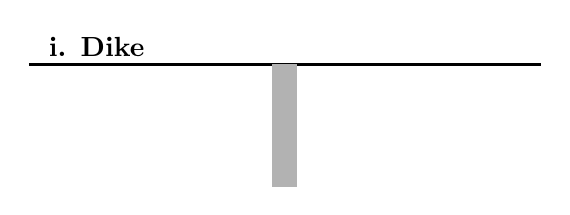
\begin{tikzpicture}[scale=0.65]
  % Label
  \node[anchor=west,font=\bfseries] at (-4.8,0.35) {i. Dike};

  % Geometry
  \draw[thick] (-5,0) -- (5,0);
  \fill[gray!60] (-0.25,0) rectangle (0.25,-2.4);
\end{tikzpicture}
\end{minipage}
\hfill
\begin{minipage}[t]{0.48\textwidth}
\centering

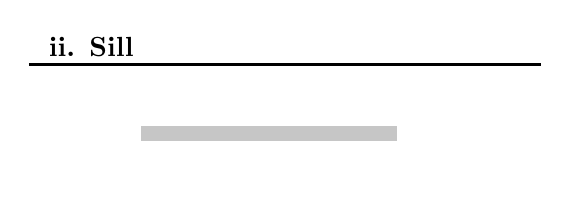
\begin{tikzpicture}[scale=0.65]
  % Label
  \node[anchor=west,font=\bfseries] at (-4.8,0.35)
        {ii. Sill};

  % Geometry
  \draw[thick] (-5,0) -- (5,0);
  \fill[gray!45] (-2.8,-1.2) rectangle (2.2,-1.5);
  \draw[thin] (-5,-2.4) -- (-5,-2.4);
\end{tikzpicture}
\end{minipage}

\vspace{1em}

% =========================
% Row 2
% =========================

\begin{minipage}[t]{0.48\textwidth}
\centering

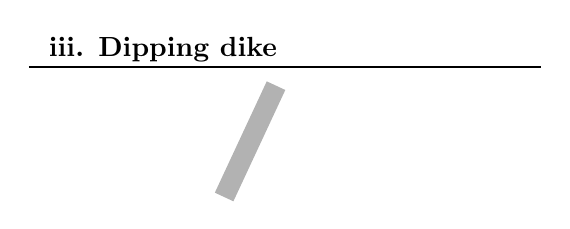
\begin{tikzpicture}[scale=0.65]
  % Label
  \node[anchor=west,font=\bfseries] at (-4.8,0.35)
        {iii. Dipping dike};

  % Geometry
  \draw[thick] (-5,0) -- (5,0);
  \begin{scope}[rotate=-25]
    \fill[gray!60] (-0.2,-0.4) rectangle (0.2,-2.8);
  \end{scope}
\end{tikzpicture}
\end{minipage}
\hfill
\begin{minipage}[t]{0.48\textwidth}
\centering

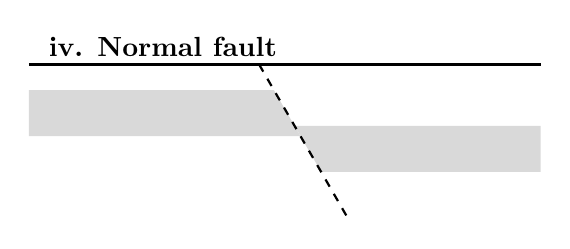
\begin{tikzpicture}[scale=0.65]
  % Label
  \node[anchor=west,font=\bfseries] at (-4.8,0.35)
        {iv. Normal fault};

  % --- Surface ---
  \draw[thick] (-5,0) -- (5,0);

  % --- Parameters ---
  \def\xf{-0.5}
  \def\dip{60}
  \def\tlay{0.9}
  \def\ztopL{-0.5}
  \def\ztopR{-1.2}

  % --- Trig helpers ---
  \pgfmathsetmacro{\cosd}{cos(\dip)}
  \pgfmathsetmacro{\sind}{sin(\dip)}
  \pgfmathsetmacro{\cotd}{\cosd/\sind}

  % --- Left block ---
  \pgfmathsetmacro{\zLt}{\ztopL}
  \pgfmathsetmacro{\zLb}{\ztopL - \tlay}
  \pgfmathsetmacro{\xLt}{\xf - (\zLt)*\cotd}
  \pgfmathsetmacro{\xLb}{\xf - (\zLb)*\cotd}

  % --- Right block ---
  \pgfmathsetmacro{\zRt}{\ztopR}
  \pgfmathsetmacro{\zRb}{\ztopR - \tlay}
  \pgfmathsetmacro{\xRt}{\xf - (\zRt)*\cotd}
  \pgfmathsetmacro{\xRb}{\xf - (\zRb)*\cotd}

  % --- Bodies ---
  \path[fill=gray!30,draw=none]
       (-5,\zLt) -- (\xLt,\zLt) -- (\xLb,\zLb) -- (-5,\zLb) -- cycle;

  \path[fill=gray!30,draw=none]
       (\xRt,\zRt) -- (5,\zRt) -- (5,\zRb) -- (\xRb,\zRb) -- cycle;

  % --- Fault ---
  \draw[dashed,thick] (\xf,0) -- ++({3.5*\cosd},{-3.5*\sind});
\end{tikzpicture}
\end{minipage}

\caption{Idealized 2-D density structures used to explore gravity anomaly geometry.}
\end{figure}

Sketch the expected gravity anomaly as a function of horizontal distance.
On each sketch, clearly indicate:
\begin{enumerate}
    \item The location of the maximum anomaly relative to the body
    \item Whether the anomaly is symmetric or asymmetric
    \item The far-field (asymptotic) behavior
\end{enumerate}

\subsection*{(B) Forward modeling}
Using the Talwani gravity modeling program (\verb+gravity2d_gui.py+) to:
\begin{enumerate}
    \item Draw polygons to match the the bodies above.
    \item Compute the gravity anomaly assuming a constant density contrast.
    \item Compare the modeled anomalies with your sketches.
    \item Explore changes in the dike model. Comment specifically on how the following changes the wavelength and amplitude:
    \begin{enumerate}
        \item depth of burial
        \item density contrast
        \item width of the body
    \end{enumerate}
\end{enumerate}

%%%%%%%%%%%%%%%%%%%%%%%%%%%%%%%%%%%%%%%%%%%%%%%%%%%%%%%%%%%%
\clearpage
\section*{Question 2: Shallow and Deep Bodies\hfill [10 pts.]}

In this question you will compute gravity anomalies using the analytic solution for
a two-dimensional body of constant density contrast, following the formulation of
Talwani et al.\ (1959). All bodies are assumed to extend infinitely perpendicular to the
$x$--$z$ plane.

\subsection*{(A) Gravity anomaly of a 2-D polygon}

For a polygon with $N$ vertices $(x_i, z_i)$ ordered clockwise,
the vertical gravity anomaly at surface point $x$ due to a body of
density contrast $\Delta\rho$ is

\[
\Delta g(x) =
2 G \Delta\rho
\sum_{i=1}^{N}
\left[
(x_i - x)\,
\ln\!\left(\frac{r_{i+1}}{r_i}\right)
+
(z_{i+1}-z_i)
\left(
\tan^{-1}\!\frac{x_{i+1}-x}{z_{i+1}}
-
\tan^{-1}\!\frac{x_i-x}{z_i}
\right)
\right],
\]

where

\[
r_i = \sqrt{(x_i - x)^2 + z_i^2}.
\]

You may assume $G = 6.67 \times 10^{-11}~\mathrm{m^3\,kg^{-1}\,s^{-2}}$.
This expression is exact for any 2-D polygonal body.

\textbf{This problem will be easiest to execute in python or matlab.}

\subsection*{(B) Triangular rift basin}

Consider a triangular shaped basin with two opposite 60\textdegree\ dipping fault planes, filled to the top with sediments.
\begin{enumerate}
    \item Compute the coordinates for a vertical offset of $5~\mathrm{km}$. Place (0,0) in the center of the basin.
    \item Use the equation above to compute the gravity anomaly.
    \item Plot $\Delta g(x)$ and identify:
    \begin{itemize}
        \item the location of the maximum gradient,
        \item the direction of asymmetry.
    \end{itemize}
\end{enumerate}


\subsection*{(C) Trapezoidal rift basin}

The trapezoid should have sloping edges comparable in dip to in part (B). Make the depth of the basin 3 km in this case with the same surface coordinates for the basin.

\begin{enumerate}
\item Compute the gravity anomaly using the polygon formula.
\item Compare the trapezoidal and triangular basin gravity models.
\item Discuss which features of the anomalies are controlled by:
  \begin{itemize}
  \item the slope of the edges,
  \item the depth extent of the body,
  \item the density contrast.
  \end{itemize}
\end{enumerate}

\subsection*{(D) Basin over a crustal root}

Model a shallow sedimentary basin overlying a deeper crustal root.
\begin{figure}[h!]
    \begin{center}
    \begin{tikzpicture}[scale=0.13]

    % Surface
    \draw[] (-30,0) -- (30,0);

    % Basin
    \draw[] (-15,0) -- (-10,-3) -- (10,-3) -- (15,0);

    % Root
    \draw[] (-30,-30) -- (-15,-30) -- (0,-40) -- (15,-30) -- (30,-30);

    % Labels
    \node at (0,2) {Surface};
    \node at (0,-5) {Basin};
    \node at (0,-25) {Root};

    % Dimensions
    \draw[<->] (-15,-28) -- (15,-28);
    \node at (0,-31) {$30~\mathrm{km}$};

    \draw[<->] (18,-40) -- (18,-30);
    \node at (24,-35) {$10~\mathrm{km}$};

    \end{tikzpicture}
    \end{center}
\end{figure}
Represent the crustal root as a triangular body with:

\begin{itemize}
\item Maximum thickness: $10~\mathrm{km}$
\item Total width: $30~\mathrm{km}$
\end{itemize}

\begin{enumerate}
\item Compute the gravity anomaly of the root alone.
\item Compute the anomaly of a shallow basin alone.
\item Combine the basin and root in a single model.
\end{enumerate}

By adjusting basin parameters (depth, width, density contrast),
determine whether a basin-only model can replicate a root-only model.

Explain what this implies about non-uniqueness in gravity interpretation.

% \subsection*{(E) Computational implementation}

% You may write a short script (or use AI assistance) to automatically generate polygon
% vertices and compute gravity anomalies using the equation above.

% Briefly describe:
% \begin{itemize}
%     \item the parameters you varied,
%     \item what aspects of the anomaly were most sensitive to geometry,
%     \item what aspects were poorly constrained.
% \end{itemize}

%%%%%%%%%%%%%%%%%%%%%%%%%%%%%%%%%%%%%%%%%%%%%%%%%%%%%%%%%%%%
\clearpage
\section*{Question 3: Isostasy — Oceanic vs Continental Lithosphere\hfill [10 pts.]}

Complete the \textbf{Ocean vs. Continent Isostasy} problem from Week 5.

You will show:
\begin{enumerate}
    \item why crust alone is insufficient to balance the columns,
    \item determine the difference in density contrast between oceanic and continental lithoshere to account for the difference in elevation, and
    \item determine the compositional change required to balance the columns.
\end{enumerate}

%%%%%%%%%%%%%%%%%%%%%%%%%%%%%%%%%%%%%%%%%%%%%%%%%%%%%%%%%%%%
\clearpage
\section*{Question 4: Isostatic Response to Erosion\hfill [10 pts.]}

Consider a hypothetical mountain belt initially in local isostatic equilibrium.
Unless otherwise stated, assume Airy isostasy and neglect flexural support.

Include all assumptions and justify your parameter choices.

\subsection*{(A) Single-layer crust (static response)}

Assume a single crustal layer of uniform density over mantle.
The initial surface elevation of the mountain belt is \(\varepsilon_0 = \SI{6100}{m}\),
and the total crustal thickness is approximately \(\sim \SI{70}{km}\).

\begin{enumerate}
    \item If \(\SI{2}{km}\) of material is eroded instantaneously from the surface,
    what is the new equilibrium surface elevation after isostatic rebound?
    \item How much total erosion is required to return the surface elevation to the
    surrounding baseline?
    \item What fraction of eroded material is replaced by isostatic rebound?
\end{enumerate}

Clearly state the densities you assume for the crust and mantle, and show all steps.

\subsection*{(B) Continuous erosion with isostatic rebound}

Now consider \emph{continuous erosion} acting simultaneously with isostatic rebound.
Assume that the erosion rate is proportional to surface elevation,

\[
\frac{dE}{dt} = k\,\varepsilon(t),
\]

where \(E(t)\) is the cumulative erosion thickness, \(\varepsilon(t)\) is the surface elevation,
and \(k\) is an erosion constant with units of inverse time.

Reasonable values for \(k\) in continental mountain belts are
\(k \sim 0.05\text{--}0.5~\mathrm{Myr^{-1}}\).
For this problem, use
\[
k = 0.1~\mathrm{Myr^{-1}}.
\]

\vspace{0.5em}

Under local isostatic equilibrium, the rate of change of surface elevation due to erosion
and rebound may be written in the general form

\[
\frac{d\varepsilon}{dt} = -\alpha \frac{dE}{dt},
\]

where \(\alpha\) depends on the isostatic model and density structure.

\begin{enumerate}
    \item Derive the value of \(\alpha\) for Airy isostasy in terms of crustal and mantle
    densities.
    \item Combine the equations above to obtain a differential equation for \(\varepsilon(t)\).
\end{enumerate}

The resulting equation has the general solution

\[
\varepsilon(t) = h_0 \exp\!\left(-\alpha k t\right),
\]

where \(h_0\) is the initial elevation at \(t=0\).

\begin{enumerate}
    \setcounter{enumi}{2}
    \item Show that in the absence of a density contrast (no rebound) the solution reduces to \(\varepsilon(t) = \varepsilon_0 \exp(- k t)\)
    \item What is the change in the initial erosion rate with and without isostasy?
    \item Using your derived value of \(\alpha\), calculate the time required to erode
    \(95\%\) of the initial relief (i.e.\ for \(\varepsilon = 0.05\,\varepsilon_0\)).
    \item Compare this timescale to the erosion-only timescale \(k^{-1}\), and explain
    physically why they differ.
    \item Briefly discuss what this simple model implies about the longevity of large
    mountain belts.
\end{enumerate}

% \subsection*{(B) Two-layer crust}
% Now assume the crust initally consists of:
% \begin{itemize}
%     \item \SI{40}{km} of granitic upper crust
%     \item \SI{30}{km} of mafic lower crust
% \end{itemize}

% Assume erosion removes only upper crustal material.

% \begin{enumerate}
%     \item Repeat the calculations from part (A).
%     \item Compare results with the single-layer case.
%     \item Discuss geological implications for long-lived mountain belts.
% \end{enumerate}

\end{document}